\section*{Conclusão}

Concluindo , esse projeto comparou quatro algoritmos de Machine Learning na tarefa de prever o resultado de suporte em um programa de horta comunitária.
O pré-processamento foi realizando cuidadosamente, com a remoção de atributos contendo alguns dados ausentes (mais de 80\% na coluna other\_support\_plans) e o uso de codificadores ordinais e nominais, foi crucial para o sucesso dos modelos.
A avaliação dos modelos foi realizada usando validação cruzada de 5 folds (5-Fold CV) para Acurácia, e uma divisão de validação (20\% dos dados) para a geração da curva AUC. Os resultados são resumidos abaixo:

\begin{center}
\begin{tabular}{lcc}
\toprule
\textbf{Modelo} & \textbf{Acurácia Média (CV)} & \textbf{AUC (Validação)} \\
\midrule
\textbf{Random Forest} & \textbf{0.7525} & \textbf{0.79} \\
Gradient Boosting & 0.7350 & 0.75 \\
Decision Tree & 0.6800 & 0.68 \\
Gaussian Naive Bayes & 0.6663 & 0.73 \\
\bottomrule
\end{tabular}
\end{center}

\subsection*{Análise dos Resultados}
Os resultados confirmam o poder dos métodos de ensemble (Random Forest e Gradient Boosting), que superaram significativamente a Árvore de Decisão única e o Naive Bayes.
O \textbf{Random Forest} foi o modelo de melhor desempenho, alcançando a maior Acurácia em validação cruzada (0.7525)  e a maior AUC (0.79) no conjunto de validação.

A Figura \ref{fig:roc_comp} demonstra visualmente a superioridade do Random Forest. Sua curva (AUC 0.79) está notavelmente mais próxima do canto superior esquerdo, indicativo de ser um melhor classificador em comparação com o Gradient Boosting (0.75), Naive Bayes (0.73) e a Árvore de Decisão (0.68).

\begin{figure}[H]
    \centering
    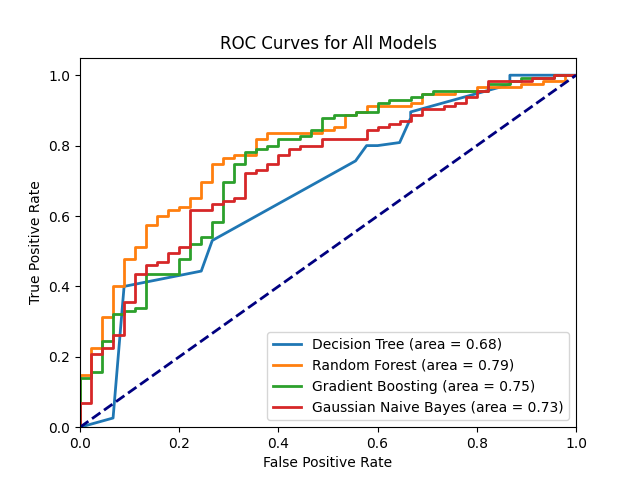
\includegraphics[width=1\linewidth]{results/all_models_roc_curve.png}
    \caption{Comparação da Curva ROC para todos os modelos no conjunto de validação.}
    \label{fig:roc_comp}
\end{figure}

\subsection*{Recomendação Final}
Por fim, com base nesta análise, recomenda-se à coordenação do Jardim Comunitário Raízes Vivas a implementação do modelo \textbf{Random Forest} para a tarefa de previsão.

Ele alcançou a maior acurácia em validação cruzada (0.7525)  e a maior AUC (0.79)  no conjunto de validação, e também pode ser treinado em paralelo., demonstrando ser o modelo mais robusto e com melhor capacidade de generalização para este problema. O arquivo de submissão final \texttt{submission.csv} foi gerado pelo Random Forest. Vale lembrar também que essa é apenas a primeira entrega do trabalho, e outros algoritmos, como as redes neurais profundas, podem ser mais efetivos para essa base de dados.